\documentclass[1p]{elsarticle_modified}
%\bibliographystyle{elsarticle-num}

%\usepackage[colorlinks]{hyperref}
%\usepackage{abbrmath_seonhwa} %\Abb, \Ascr, \Acal ,\Abf, \Afrak
\usepackage{amsfonts}
\usepackage{amssymb}
\usepackage{amsmath}
\usepackage{amsthm}
\usepackage{scalefnt}
\usepackage{amsbsy}
\usepackage{kotex}
\usepackage{caption}
\usepackage{subfig}
\usepackage{color}
\usepackage{graphicx}
\usepackage{xcolor} %% white, black, red, green, blue, cyan, magenta, yellow
\usepackage{float}
\usepackage{setspace}
\usepackage{hyperref}

\usepackage{tikz}
\usetikzlibrary{arrows}

\usepackage{multirow}
\usepackage{array} % fixed length table
\usepackage{hhline}

%%%%%%%%%%%%%%%%%%%%%
\makeatletter
\renewcommand*\env@matrix[1][\arraystretch]{%
	\edef\arraystretch{#1}%
	\hskip -\arraycolsep
	\let\@ifnextchar\new@ifnextchar
	\array{*\c@MaxMatrixCols c}}
\makeatother %https://tex.stackexchange.com/questions/14071/how-can-i-increase-the-line-spacing-in-a-matrix
%%%%%%%%%%%%%%%

\usepackage[normalem]{ulem}

\newcommand{\msout}[1]{\ifmmode\text{\sout{\ensuremath{#1}}}\else\sout{#1}\fi}
%SOURCE: \msout is \stkout macro in https://tex.stackexchange.com/questions/20609/strikeout-in-math-mode

\newcommand{\cancel}[1]{
	\ifmmode
	{\color{red}\msout{#1}}
	\else
	{\color{red}\sout{#1}}
	\fi
}

\newcommand{\add}[1]{
	{\color{blue}\uwave{#1}}
}

\newcommand{\replace}[2]{
	\ifmmode
	{\color{red}\msout{#1}}{\color{blue}\uwave{#2}}
	\else
	{\color{red}\sout{#1}}{\color{blue}\uwave{#2}}
	\fi
}

\newcommand{\Sol}{\mathcal{S}} %segment
\newcommand{\D}{D} %diagram
\newcommand{\A}{\mathcal{A}} %arc


%%%%%%%%%%%%%%%%%%%%%%%%%%%%%5 test

\def\sl{\operatorname{\textup{SL}}(2,\Cbb)}
\def\psl{\operatorname{\textup{PSL}}(2,\Cbb)}
\def\quan{\mkern 1mu \triangleright \mkern 1mu}

\theoremstyle{definition}
\newtheorem{thm}{Theorem}[section]
\newtheorem{prop}[thm]{Proposition}
\newtheorem{lem}[thm]{Lemma}
\newtheorem{ques}[thm]{Question}
\newtheorem{cor}[thm]{Corollary}
\newtheorem{defn}[thm]{Definition}
\newtheorem{exam}[thm]{Example}
\newtheorem{rmk}[thm]{Remark}
\newtheorem{alg}[thm]{Algorithm}

\newcommand{\I}{\sqrt{-1}}
\begin{document}

%\begin{frontmatter}
%
%\title{Boundary parabolic representations of knots up to 8 crossings}
%
%%% Group authors per affiliation:
%\author{Yunhi Cho} 
%\address{Department of Mathematics, University of Seoul, Seoul, Korea}
%\ead{yhcho@uos.ac.kr}
%
%
%\author{Seonhwa Kim} %\fnref{s_kim}}
%\address{Center for Geometry and Physics, Institute for Basic Science, Pohang, 37673, Korea}
%\ead{ryeona17@ibs.re.kr}
%
%\author{Hyuk Kim}
%\address{Department of Mathematical Sciences, Seoul National University, Seoul 08826, Korea}
%\ead{hyukkim@snu.ac.kr}
%
%\author{Seokbeom Yoon}
%\address{Department of Mathematical Sciences, Seoul National University, Seoul, 08826,  Korea}
%\ead{sbyoon15@snu.ac.kr}
%
%\begin{abstract}
%We find all boundary parabolic representation of knots up to 8 crossings.
%
%\end{abstract}
%\begin{keyword}
%    \MSC[2010] 57M25 
%\end{keyword}
%
%\end{frontmatter}

%\linenumbers
%\tableofcontents
%
\newcommand\colored[1]{\textcolor{white}{\rule[-0.35ex]{0.8em}{1.4ex}}\kern-0.8em\color{red} #1}%
%\newcommand\colored[1]{\textcolor{white}{ #1}\kern-2.17ex	\textcolor{white}{ #1}\kern-1.81ex	\textcolor{white}{ #1}\kern-2.15ex\color{red}#1	}

{\Large $\underline{12a_{1097}~(K12a_{1097})}$}

\setlength{\tabcolsep}{10pt}
\renewcommand{\arraystretch}{1.6}
\vspace{1cm}\begin{tabular}{m{100pt}>{\centering\arraybackslash}m{274pt}}
\multirow{5}{120pt}{
	\centering
	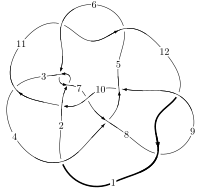
\includegraphics[width=112pt]{../../../GIT/diagram.site/Diagrams/png/1898_12a_1097.png}\\
\ \ \ A knot diagram\footnotemark}&
\allowdisplaybreaks
\textbf{Linearized knot diagam} \\
\cline{2-2}
 &
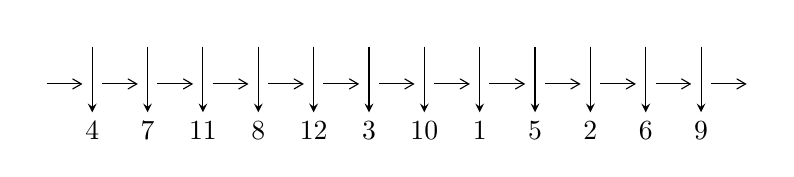
\begin{tikzpicture}[x=20pt, y=17pt]
	% nodes
	\node (C0) at (0, 0) {};
	\node (C1) at (1, 0) {};
	\node (C1U) at (1, +1) {};
	\node (C1D) at (1, -1) {4};

	\node (C2) at (2, 0) {};
	\node (C2U) at (2, +1) {};
	\node (C2D) at (2, -1) {7};

	\node (C3) at (3, 0) {};
	\node (C3U) at (3, +1) {};
	\node (C3D) at (3, -1) {11};

	\node (C4) at (4, 0) {};
	\node (C4U) at (4, +1) {};
	\node (C4D) at (4, -1) {8};

	\node (C5) at (5, 0) {};
	\node (C5U) at (5, +1) {};
	\node (C5D) at (5, -1) {12};

	\node (C6) at (6, 0) {};
	\node (C6U) at (6, +1) {};
	\node (C6D) at (6, -1) {3};

	\node (C7) at (7, 0) {};
	\node (C7U) at (7, +1) {};
	\node (C7D) at (7, -1) {10};

	\node (C8) at (8, 0) {};
	\node (C8U) at (8, +1) {};
	\node (C8D) at (8, -1) {1};

	\node (C9) at (9, 0) {};
	\node (C9U) at (9, +1) {};
	\node (C9D) at (9, -1) {5};

	\node (C10) at (10, 0) {};
	\node (C10U) at (10, +1) {};
	\node (C10D) at (10, -1) {2};

	\node (C11) at (11, 0) {};
	\node (C11U) at (11, +1) {};
	\node (C11D) at (11, -1) {6};

	\node (C12) at (12, 0) {};
	\node (C12U) at (12, +1) {};
	\node (C12D) at (12, -1) {9};
	\node (C13) at (13, 0) {};

	% arrows
	\draw[->,>={angle 60}]
	(C0) edge (C1) (C1) edge (C2) (C2) edge (C3) (C3) edge (C4) (C4) edge (C5) (C5) edge (C6) (C6) edge (C7) (C7) edge (C8) (C8) edge (C9) (C9) edge (C10) (C10) edge (C11) (C11) edge (C12) (C12) edge (C13) ;	\draw[->,>=stealth]
	(C1U) edge (C1D) (C2U) edge (C2D) (C3U) edge (C3D) (C4U) edge (C4D) (C5U) edge (C5D) (C6U) edge (C6D) (C7U) edge (C7D) (C8U) edge (C8D) (C9U) edge (C9D) (C10U) edge (C10D) (C11U) edge (C11D) (C12U) edge (C12D) ;
	\end{tikzpicture} \\
\hhline{~~} \\& 
\textbf{Solving Sequence} \\ \cline{2-2} 
 &
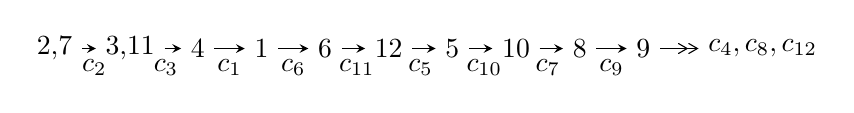
\begin{tikzpicture}[x=23pt, y=7pt]
	% node
	\node (A0) at (-1/8, 0) {2,7};
	\node (A1) at (17/16, 0) {3,11};
	\node (A2) at (17/8, 0) {4};
	\node (A3) at (25/8, 0) {1};
	\node (A4) at (33/8, 0) {6};
	\node (A5) at (41/8, 0) {12};
	\node (A6) at (49/8, 0) {5};
	\node (A7) at (57/8, 0) {10};
	\node (A8) at (65/8, 0) {8};
	\node (A9) at (73/8, 0) {9};
	\node (C1) at (1/2, -1) {$c_{2}$};
	\node (C2) at (13/8, -1) {$c_{3}$};
	\node (C3) at (21/8, -1) {$c_{1}$};
	\node (C4) at (29/8, -1) {$c_{6}$};
	\node (C5) at (37/8, -1) {$c_{11}$};
	\node (C6) at (45/8, -1) {$c_{5}$};
	\node (C7) at (53/8, -1) {$c_{10}$};
	\node (C8) at (61/8, -1) {$c_{7}$};
	\node (C9) at (69/8, -1) {$c_{9}$};
	\node (A10) at (11, 0) {$c_{4},c_{8},c_{12}$};

	% edge
	\draw[->,>=stealth]	
	(A0) edge (A1) (A1) edge (A2) (A2) edge (A3) (A3) edge (A4) (A4) edge (A5) (A5) edge (A6) (A6) edge (A7) (A7) edge (A8) (A8) edge (A9) ;
	\draw[->>,>={angle 60}]	
	(A9) edge (A10);
\end{tikzpicture} \\ 

\end{tabular} \\

\footnotetext{
The image of knot diagram is generated by the software ``\textbf{Draw programme}" developed by Andrew Bartholomew(\url{http://www.layer8.co.uk/maths/draw/index.htm\#Running-draw}), where we modified some parts for our purpose(\url{https://github.com/CATsTAILs/LinksPainter}).
}\phantom \\ \newline 
\centering \textbf{Ideals for irreducible components\footnotemark of $X_{\text{par}}$} 
 
\begin{align*}
I^u_{1}&=\langle 
-3102178454 u^{24}-15488927339 u^{23}+\cdots+126671695426 b-3208274034,\\
\phantom{I^u_{1}}&\phantom{= \langle  }-109125500312 u^{24}+169518693654 u^{23}+\cdots+126671695426 a+248511754619,\\
\phantom{I^u_{1}}&\phantom{= \langle  }u^{25}- u^{24}+\cdots-4 u-1\rangle \\
I^u_{2}&=\langle 
-3.64244\times10^{488} u^{119}-1.96796\times10^{488} u^{118}+\cdots+1.15571\times10^{490} b-2.23233\times10^{491},\\
\phantom{I^u_{2}}&\phantom{= \langle  }2.53470\times10^{491} u^{119}+1.70055\times10^{491} u^{118}+\cdots+4.31080\times10^{492} a+3.08118\times10^{494},\\
\phantom{I^u_{2}}&\phantom{= \langle  }u^{120}+u^{119}+\cdots+3274 u+373\rangle \\
I^u_{3}&=\langle 
-1.26770\times10^{32} u^{33}-6.32813\times10^{32} u^{32}+\cdots+1.13470\times10^{33} b-1.22256\times10^{33},\\
\phantom{I^u_{3}}&\phantom{= \langle  }8.99358\times10^{32} u^{33}+2.58920\times10^{33} u^{32}+\cdots+7.94293\times10^{33} a-1.81454\times10^{34},\;u^{34}+4 u^{33}+\cdots+10 u+7\rangle \\
I^u_{4}&=\langle 
u^2+b- u+1,\;a+u,\;u^3- u^2+2 u-1\rangle \\
\\
\end{align*}
\raggedright * 4 irreducible components of $\dim_{\mathbb{C}}=0$, with total 182 representations.\\
\footnotetext{All coefficients of polynomials are rational numbers. But the coefficients are sometimes approximated in decimal forms when there is not enough margin.}
\newpage
\renewcommand{\arraystretch}{1}
\centering \section*{I. $I^u_{1}= \langle -3.10\times10^{9} u^{24}-1.55\times10^{10} u^{23}+\cdots+1.27\times10^{11} b-3.21\times10^{9},\;-1.09\times10^{11} u^{24}+1.70\times10^{11} u^{23}+\cdots+1.27\times10^{11} a+2.49\times10^{11},\;u^{25}- u^{24}+\cdots-4 u-1 \rangle$}
\flushleft \textbf{(i) Arc colorings}\\
\begin{tabular}{m{7pt} m{180pt} m{7pt} m{180pt} }
\flushright $a_{2}=$&$\begin{pmatrix}1\\0\end{pmatrix}$ \\
\flushright $a_{7}=$&$\begin{pmatrix}0\\u\end{pmatrix}$ \\
\flushright $a_{3}=$&$\begin{pmatrix}1\\u^2\end{pmatrix}$ \\
\flushright $a_{11}=$&$\begin{pmatrix}0.861483 u^{24}-1.33825 u^{23}+\cdots-10.2790 u-1.96186\\0.0244899 u^{24}+0.122276 u^{23}+\cdots+1.96923 u+0.0253275\end{pmatrix}$ \\
\flushright $a_{4}=$&$\begin{pmatrix}-1.24527 u^{24}+1.18630 u^{23}+\cdots+4.94727 u+5.83862\\0.330003 u^{24}-0.336309 u^{23}+\cdots-1.60736 u-0.885973\end{pmatrix}$ \\
\flushright $a_{1}=$&$\begin{pmatrix}-1.04759 u^{24}+1.71210 u^{23}+\cdots+8.80196 u+2.26840\\0.0958880 u^{24}-0.387211 u^{23}+\cdots-0.961789 u+0.417723\end{pmatrix}$ \\
\flushright $a_{6}=$&$\begin{pmatrix}u\\u^3+u\end{pmatrix}$ \\
\flushright $a_{12}=$&$\begin{pmatrix}1.20401 u^{24}-1.61811 u^{23}+\cdots-11.3742 u-2.51518\\0.0593353 u^{24}+0.0734059 u^{23}+\cdots+1.46726 u-0.465323\end{pmatrix}$ \\
\flushright $a_{5}=$&$\begin{pmatrix}-0.889942 u^{24}+0.849149 u^{23}+\cdots-1.21154 u+5.82056\\0.166699 u^{24}-0.468616 u^{23}+\cdots-0.00571945 u-1.23391\end{pmatrix}$ \\
\flushright $a_{10}=$&$\begin{pmatrix}0.885973 u^{24}-1.21598 u^{23}+\cdots-8.30975 u-1.93653\\0.0244899 u^{24}+0.122276 u^{23}+\cdots+1.96923 u+0.0253275\end{pmatrix}$ \\
\flushright $a_{8}=$&$\begin{pmatrix}0.417723 u^{24}-0.321835 u^{23}+\cdots+1.89594 u-2.63268\\-0.338923 u^{24}+0.558319 u^{23}+\cdots+0.971046 u+0.791762\end{pmatrix}$ \\
\flushright $a_{9}=$&$\begin{pmatrix}-0.246780 u^{24}+0.403197 u^{23}+\cdots+3.81792 u-1.58508\\-0.0476005 u^{24}+0.202824 u^{23}+\cdots+0.169772 u+0.695874\end{pmatrix}$\\&\end{tabular}
\flushleft \textbf{(ii) Obstruction class $= -1$}\\~\\
\flushleft \textbf{(iii) Cusp Shapes $= \frac{58456314520}{63335847713} u^{24}-\frac{118830395739}{63335847713} u^{23}+\cdots-\frac{1160180780406}{63335847713} u-\frac{761638158750}{63335847713}$}\\~\\
\newpage\renewcommand{\arraystretch}{1}
\flushleft \textbf{(iv) u-Polynomials at the component}\newline \\
\begin{tabular}{m{50pt}|m{274pt}}
Crossings & \hspace{64pt}u-Polynomials at each crossing \\
\hline $$\begin{aligned}c_{1},c_{7}\end{aligned}$$&$\begin{aligned}
&u^{25}- u^{24}+\cdots+28 u+13
\end{aligned}$\\
\hline $$\begin{aligned}c_{2},c_{6},c_{8}\\c_{12}\end{aligned}$$&$\begin{aligned}
&u^{25}+u^{24}+\cdots-4 u+1
\end{aligned}$\\
\hline $$\begin{aligned}c_{3},c_{9}\end{aligned}$$&$\begin{aligned}
&u^{25}- u^{24}+\cdots+24 u+8
\end{aligned}$\\
\hline $$\begin{aligned}c_{4},c_{10}\end{aligned}$$&$\begin{aligned}
&4(4 u^{25}-4 u^{24}+\cdots+4 u+1)
\end{aligned}$\\
\hline $$\begin{aligned}c_{5},c_{11}\end{aligned}$$&$\begin{aligned}
&4(4 u^{25}-12 u^{24}+\cdots-344 u+40)
\end{aligned}$\\
\hline
\end{tabular}\\~\\
\newpage\renewcommand{\arraystretch}{1}
\flushleft \textbf{(v) Riley Polynomials at the component}\newline \\
\begin{tabular}{m{50pt}|m{274pt}}
Crossings & \hspace{64pt}Riley Polynomials at each crossing \\
\hline $$\begin{aligned}c_{1},c_{7}\end{aligned}$$&$\begin{aligned}
&y^{25}+21 y^{24}+\cdots+4112 y-169
\end{aligned}$\\
\hline $$\begin{aligned}c_{2},c_{6},c_{8}\\c_{12}\end{aligned}$$&$\begin{aligned}
&y^{25}+17 y^{24}+\cdots+20 y-1
\end{aligned}$\\
\hline $$\begin{aligned}c_{3},c_{9}\end{aligned}$$&$\begin{aligned}
&y^{25}+9 y^{24}+\cdots+256 y-64
\end{aligned}$\\
\hline $$\begin{aligned}c_{4},c_{10}\end{aligned}$$&$\begin{aligned}
&16(16 y^{25}+336 y^{24}+\cdots-4 y-1)
\end{aligned}$\\
\hline $$\begin{aligned}c_{5},c_{11}\end{aligned}$$&$\begin{aligned}
&16(16 y^{25}+304 y^{24}+\cdots+27776 y-1600)
\end{aligned}$\\
\hline
\end{tabular}\\~\\
\newpage\flushleft \textbf{(vi) Complex Volumes and Cusp Shapes}
$$\begin{array}{c|c|c}  
\text{Solutions to }I^u_{1}& \I (\text{vol} + \sqrt{-1}CS) & \text{Cusp shape}\\
 \hline 
\begin{aligned}
u &= \phantom{-}0.211687 + 0.985151 I \\
a &= \phantom{-}0.054135 - 1.103940 I \\
b &= -0.144638 + 0.502780 I\end{aligned}
 & \phantom{-}2.32892 - 2.20108 I & -10.08383 + 3.97912 I \\ \hline\begin{aligned}
u &= \phantom{-}0.211687 - 0.985151 I \\
a &= \phantom{-}0.054135 + 1.103940 I \\
b &= -0.144638 - 0.502780 I\end{aligned}
 & \phantom{-}2.32892 + 2.20108 I & -10.08383 - 3.97912 I \\ \hline\begin{aligned}
u &= \phantom{-}0.531651 + 0.812171 I \\
a &= -0.650095 - 0.103642 I \\
b &= -0.575312 - 0.511008 I\end{aligned}
 & \phantom{-}1.67097 - 3.94275 I & -14.2459 + 7.3928 I \\ \hline\begin{aligned}
u &= \phantom{-}0.531651 - 0.812171 I \\
a &= -0.650095 + 0.103642 I \\
b &= -0.575312 + 0.511008 I\end{aligned}
 & \phantom{-}1.67097 + 3.94275 I & -14.2459 - 7.3928 I \\ \hline\begin{aligned}
u &= -0.090278 + 1.083730 I \\
a &= \phantom{-}0.34542 + 2.11090 I \\
b &= \phantom{-}0.55243 - 1.97550 I\end{aligned}
 & \phantom{-}6.61385 + 1.08919 I & -3.90952 + 2.05372 I \\ \hline\begin{aligned}
u &= -0.090278 - 1.083730 I \\
a &= \phantom{-}0.34542 - 2.11090 I \\
b &= \phantom{-}0.55243 + 1.97550 I\end{aligned}
 & \phantom{-}6.61385 - 1.08919 I & -3.90952 - 2.05372 I \\ \hline\begin{aligned}
u &= -0.759076 + 0.841792 I \\
a &= \phantom{-}0.983474 - 0.029586 I \\
b &= \phantom{-}0.082128 - 0.598891 I\end{aligned}
 & \phantom{-}4.59853 + 2.71316 I & -3.58633 - 2.16462 I \\ \hline\begin{aligned}
u &= -0.759076 - 0.841792 I \\
a &= \phantom{-}0.983474 + 0.029586 I \\
b &= \phantom{-}0.082128 + 0.598891 I\end{aligned}
 & \phantom{-}4.59853 - 2.71316 I & -3.58633 + 2.16462 I \\ \hline\begin{aligned}
u &= -0.795867 + 0.037941 I \\
a &= -0.090425 + 0.410318 I \\
b &= \phantom{-}0.678970 + 0.915805 I\end{aligned}
 & \phantom{-}0.07267 - 4.35672 I & -13.6982 + 5.9671 I \\ \hline\begin{aligned}
u &= -0.795867 - 0.037941 I \\
a &= -0.090425 - 0.410318 I \\
b &= \phantom{-}0.678970 - 0.915805 I\end{aligned}
 & \phantom{-}0.07267 + 4.35672 I & -13.6982 - 5.9671 I\\
 \hline 
 \end{array}$$\newpage$$\begin{array}{c|c|c}  
\text{Solutions to }I^u_{1}& \I (\text{vol} + \sqrt{-1}CS) & \text{Cusp shape}\\
 \hline 
\begin{aligned}
u &= -0.130652 + 1.262320 I \\
a &= -0.36503 + 2.00469 I \\
b &= -0.262641 - 1.153140 I\end{aligned}
 & \phantom{-}11.96210 + 3.79673 I & \phantom{-}0.99019 - 1.08851 I \\ \hline\begin{aligned}
u &= -0.130652 - 1.262320 I \\
a &= -0.36503 - 2.00469 I \\
b &= -0.262641 + 1.153140 I\end{aligned}
 & \phantom{-}11.96210 - 3.79673 I & \phantom{-}0.99019 + 1.08851 I \\ \hline\begin{aligned}
u &= \phantom{-}1.283170 + 0.138278 I \\
a &= -0.1264500 + 0.0272136 I \\
b &= -0.609786 - 1.030790 I\end{aligned}
 & \phantom{-}5.09693 - 7.29373 I & -6.53712 + 7.10526 I \\ \hline\begin{aligned}
u &= \phantom{-}1.283170 - 0.138278 I \\
a &= -0.1264500 - 0.0272136 I \\
b &= -0.609786 + 1.030790 I\end{aligned}
 & \phantom{-}5.09693 + 7.29373 I & -6.53712 - 7.10526 I \\ \hline\begin{aligned}
u &= -0.324609 + 1.255330 I \\
a &= \phantom{-}0.174379 - 1.064750 I \\
b &= \phantom{-}0.205309 + 0.235499 I\end{aligned}
 & \phantom{-}8.79693 + 5.43785 I & -7.61088 - 4.32634 I \\ \hline\begin{aligned}
u &= -0.324609 - 1.255330 I \\
a &= \phantom{-}0.174379 + 1.064750 I \\
b &= \phantom{-}0.205309 - 0.235499 I\end{aligned}
 & \phantom{-}8.79693 - 5.43785 I & -7.61088 + 4.32634 I \\ \hline\begin{aligned}
u &= -0.420644 + 1.280190 I \\
a &= -0.04988 - 1.77342 I \\
b &= -1.01226 + 1.62483 I\end{aligned}
 & \phantom{-}7.8259 + 13.3271 I & -5.74524 - 10.07551 I \\ \hline\begin{aligned}
u &= -0.420644 - 1.280190 I \\
a &= -0.04988 + 1.77342 I \\
b &= -1.01226 - 1.62483 I\end{aligned}
 & \phantom{-}7.8259 - 13.3271 I & -5.74524 + 10.07551 I \\ \hline\begin{aligned}
u &= \phantom{-}0.50923 + 1.46306 I \\
a &= \phantom{-}0.08105 - 1.50897 I \\
b &= \phantom{-}1.07565 + 1.36286 I\end{aligned}
 & \phantom{-}15.4595 - 19.6209 I & -4.50944 + 9.03245 I \\ \hline\begin{aligned}
u &= \phantom{-}0.50923 - 1.46306 I \\
a &= \phantom{-}0.08105 + 1.50897 I \\
b &= \phantom{-}1.07565 - 1.36286 I\end{aligned}
 & \phantom{-}15.4595 + 19.6209 I & -4.50944 - 9.03245 I\\
 \hline 
 \end{array}$$\newpage$$\begin{array}{c|c|c}  
\text{Solutions to }I^u_{1}& \I (\text{vol} + \sqrt{-1}CS) & \text{Cusp shape}\\
 \hline 
\begin{aligned}
u &= \phantom{-}0.56756 + 1.47388 I \\
a &= -0.495606 + 0.843370 I \\
b &= -0.002290 - 1.336230 I\end{aligned}
 & \phantom{-}14.1477 - 6.4090 I & -0.73994 + 3.70265 I \\ \hline\begin{aligned}
u &= \phantom{-}0.56756 - 1.47388 I \\
a &= -0.495606 - 0.843370 I \\
b &= -0.002290 + 1.336230 I\end{aligned}
 & \phantom{-}14.1477 + 6.4090 I & -0.73994 - 3.70265 I \\ \hline\begin{aligned}
u &= \phantom{-}0.303142\phantom{ +0.000000I} \\
a &= -0.873492\phantom{ +0.000000I} \\
b &= \phantom{-}0.266168\phantom{ +0.000000I}\end{aligned}
 & -0.553708\phantom{ +0.000000I} & -17.9600\phantom{ +0.000000I} \\ \hline\begin{aligned}
u &= -0.233731 + 0.135219 I \\
a &= \phantom{-}1.57579 - 3.69840 I \\
b &= -0.620642 + 0.604636 I\end{aligned}
 & \phantom{-}3.94965 + 0.82098 I & -7.34374 - 4.35501 I \\ \hline\begin{aligned}
u &= -0.233731 - 0.135219 I \\
a &= \phantom{-}1.57579 + 3.69840 I \\
b &= -0.620642 - 0.604636 I\end{aligned}
 & \phantom{-}3.94965 - 0.82098 I & -7.34374 + 4.35501 I\\
 \hline 
 \end{array}$$\newpage\newpage\renewcommand{\arraystretch}{1}
\centering \section*{II. $I^u_{2}= \langle -3.64\times10^{488} u^{119}-1.97\times10^{488} u^{118}+\cdots+1.16\times10^{490} b-2.23\times10^{491},\;2.53\times10^{491} u^{119}+1.70\times10^{491} u^{118}+\cdots+4.31\times10^{492} a+3.08\times10^{494},\;u^{120}+u^{119}+\cdots+3274 u+373 \rangle$}
\flushleft \textbf{(i) Arc colorings}\\
\begin{tabular}{m{7pt} m{180pt} m{7pt} m{180pt} }
\flushright $a_{2}=$&$\begin{pmatrix}1\\0\end{pmatrix}$ \\
\flushright $a_{7}=$&$\begin{pmatrix}0\\u\end{pmatrix}$ \\
\flushright $a_{3}=$&$\begin{pmatrix}1\\u^2\end{pmatrix}$ \\
\flushright $a_{11}=$&$\begin{pmatrix}-0.0587990 u^{119}-0.0394486 u^{118}+\cdots-331.889 u-71.4760\\0.0315169 u^{119}+0.0170282 u^{118}+\cdots+82.3482 u+19.3157\end{pmatrix}$ \\
\flushright $a_{4}=$&$\begin{pmatrix}0.00530998 u^{119}-0.0270182 u^{118}+\cdots-221.501 u-36.6777\\0.0182302 u^{119}+0.0140764 u^{118}+\cdots+116.691 u+21.9513\end{pmatrix}$ \\
\flushright $a_{1}=$&$\begin{pmatrix}-0.160110 u^{119}-0.129560 u^{118}+\cdots-888.759 u-170.800\\0.0324386 u^{119}+0.0221919 u^{118}+\cdots+236.973 u+50.2961\end{pmatrix}$ \\
\flushright $a_{6}=$&$\begin{pmatrix}u\\u^3+u\end{pmatrix}$ \\
\flushright $a_{12}=$&$\begin{pmatrix}-0.0431920 u^{119}-0.0375647 u^{118}+\cdots-393.968 u-82.1957\\0.0191721 u^{119}+0.0140410 u^{118}+\cdots+59.3771 u+13.7147\end{pmatrix}$ \\
\flushright $a_{5}=$&$\begin{pmatrix}0.00557811 u^{119}+0.0117214 u^{118}+\cdots-16.7458 u+0.784071\\-0.00709475 u^{119}-0.0228846 u^{118}+\cdots+16.8580 u+7.18962\end{pmatrix}$ \\
\flushright $a_{10}=$&$\begin{pmatrix}-0.0272820 u^{119}-0.0224204 u^{118}+\cdots-249.541 u-52.1603\\0.0315169 u^{119}+0.0170282 u^{118}+\cdots+82.3482 u+19.3157\end{pmatrix}$ \\
\flushright $a_{8}=$&$\begin{pmatrix}0.0200896 u^{119}+0.0432169 u^{118}+\cdots+49.2589 u-5.99909\\-0.00989759 u^{119}-0.0141728 u^{118}+\cdots-7.10394 u-1.44063\end{pmatrix}$ \\
\flushright $a_{9}=$&$\begin{pmatrix}0.0982715 u^{119}+0.0637556 u^{118}+\cdots+617.329 u+129.828\\-0.00409398 u^{119}-0.00734538 u^{118}+\cdots-21.4414 u-3.91955\end{pmatrix}$\\&\end{tabular}
\flushleft \textbf{(ii) Obstruction class $= -1$}\\~\\
\flushleft \textbf{(iii) Cusp Shapes $= 0.0416181 u^{119}+0.115712 u^{118}+\cdots+275.820 u+38.7552$}\\~\\
\newpage\renewcommand{\arraystretch}{1}
\flushleft \textbf{(iv) u-Polynomials at the component}\newline \\
\begin{tabular}{m{50pt}|m{274pt}}
Crossings & \hspace{64pt}u-Polynomials at each crossing \\
\hline $$\begin{aligned}c_{1},c_{7}\end{aligned}$$&$\begin{aligned}
&u^{120}-11 u^{119}+\cdots-7076832991 u+1201214753
\end{aligned}$\\
\hline $$\begin{aligned}c_{2},c_{6},c_{8}\\c_{12}\end{aligned}$$&$\begin{aligned}
&u^{120}- u^{119}+\cdots-3274 u+373
\end{aligned}$\\
\hline $$\begin{aligned}c_{3},c_{9}\end{aligned}$$&$\begin{aligned}
&u^{120}- u^{119}+\cdots+40633750 u+2972977
\end{aligned}$\\
\hline $$\begin{aligned}c_{4},c_{10}\end{aligned}$$&$\begin{aligned}
&u^{120}+5 u^{119}+\cdots-257509 u+235151
\end{aligned}$\\
\hline $$\begin{aligned}c_{5},c_{11}\end{aligned}$$&$\begin{aligned}
&(u^{60}+6 u^{59}+\cdots+58 u+13)^{2}
\end{aligned}$\\
\hline
\end{tabular}\\~\\
\newpage\renewcommand{\arraystretch}{1}
\flushleft \textbf{(v) Riley Polynomials at the component}\newline \\
\begin{tabular}{m{50pt}|m{274pt}}
Crossings & \hspace{64pt}Riley Polynomials at each crossing \\
\hline $$\begin{aligned}c_{1},c_{7}\end{aligned}$$&$\begin{aligned}
&y^{120}+55 y^{119}+\cdots+4.74\times10^{19} y+1.44\times10^{18}
\end{aligned}$\\
\hline $$\begin{aligned}c_{2},c_{6},c_{8}\\c_{12}\end{aligned}$$&$\begin{aligned}
&y^{120}+89 y^{119}+\cdots-413086 y+139129
\end{aligned}$\\
\hline $$\begin{aligned}c_{3},c_{9}\end{aligned}$$&$\begin{aligned}
&y^{120}+71 y^{119}+\cdots+487658353656878 y+8838592242529
\end{aligned}$\\
\hline $$\begin{aligned}c_{4},c_{10}\end{aligned}$$&$\begin{aligned}
&y^{120}+71 y^{119}+\cdots+3045613958149 y+55295992801
\end{aligned}$\\
\hline $$\begin{aligned}c_{5},c_{11}\end{aligned}$$&$\begin{aligned}
&(y^{60}+38 y^{59}+\cdots-2298 y+169)^{2}
\end{aligned}$\\
\hline
\end{tabular}\\~\\
\newpage\flushleft \textbf{(vi) Complex Volumes and Cusp Shapes}
$$\begin{array}{c|c|c}  
\text{Solutions to }I^u_{2}& \I (\text{vol} + \sqrt{-1}CS) & \text{Cusp shape}\\
 \hline 
\begin{aligned}
u &= -0.176278 + 1.003150 I \\
a &= -0.26302 + 1.69210 I \\
b &= \phantom{-}0.702847 - 0.582113 I\end{aligned}
 & -0.45517 + 1.61974 I & \phantom{-0.000000 } 0 \\ \hline\begin{aligned}
u &= -0.176278 - 1.003150 I \\
a &= -0.26302 - 1.69210 I \\
b &= \phantom{-}0.702847 + 0.582113 I\end{aligned}
 & -0.45517 - 1.61974 I & \phantom{-0.000000 } 0 \\ \hline\begin{aligned}
u &= \phantom{-}0.668703 + 0.773478 I \\
a &= -1.38571 + 0.91884 I \\
b &= -1.082060 + 0.140425 I\end{aligned}
 & \phantom{-}2.66044 - 2.58613 I & \phantom{-0.000000 } 0 \\ \hline\begin{aligned}
u &= \phantom{-}0.668703 - 0.773478 I \\
a &= -1.38571 - 0.91884 I \\
b &= -1.082060 - 0.140425 I\end{aligned}
 & \phantom{-}2.66044 + 2.58613 I & \phantom{-0.000000 } 0 \\ \hline\begin{aligned}
u &= \phantom{-}0.109634 + 1.023630 I \\
a &= -0.33741 + 5.27176 I \\
b &= -0.63155 - 5.30275 I\end{aligned}
 & \phantom{-}6.56424\phantom{ +0.000000I} & \phantom{-0.000000 } 0 \\ \hline\begin{aligned}
u &= \phantom{-}0.109634 - 1.023630 I \\
a &= -0.33741 - 5.27176 I \\
b &= -0.63155 + 5.30275 I\end{aligned}
 & \phantom{-}6.56424\phantom{ +0.000000I} & \phantom{-0.000000 } 0 \\ \hline\begin{aligned}
u &= -0.333875 + 0.882085 I \\
a &= \phantom{-}0.39883 + 1.37895 I \\
b &= \phantom{-}1.152120 - 0.113139 I\end{aligned}
 & -1.10643 + 1.49905 I & \phantom{-0.000000 } 0 \\ \hline\begin{aligned}
u &= -0.333875 - 0.882085 I \\
a &= \phantom{-}0.39883 - 1.37895 I \\
b &= \phantom{-}1.152120 + 0.113139 I\end{aligned}
 & -1.10643 - 1.49905 I & \phantom{-0.000000 } 0 \\ \hline\begin{aligned}
u &= -0.982492 + 0.426289 I \\
a &= \phantom{-}0.0810181 - 0.1157020 I \\
b &= -0.598200 + 0.684462 I\end{aligned}
 & \phantom{-}3.68720 + 3.23259 I & \phantom{-0.000000 } 0 \\ \hline\begin{aligned}
u &= -0.982492 - 0.426289 I \\
a &= \phantom{-}0.0810181 + 0.1157020 I \\
b &= -0.598200 - 0.684462 I\end{aligned}
 & \phantom{-}3.68720 - 3.23259 I & \phantom{-0.000000 } 0\\
 \hline 
 \end{array}$$\newpage$$\begin{array}{c|c|c}  
\text{Solutions to }I^u_{2}& \I (\text{vol} + \sqrt{-1}CS) & \text{Cusp shape}\\
 \hline 
\begin{aligned}
u &= -0.369669 + 1.016010 I \\
a &= \phantom{-}0.952924 + 0.891255 I \\
b &= -0.494773 - 0.424758 I\end{aligned}
 & \phantom{-}4.55693 + 1.81266 I & \phantom{-0.000000 } 0 \\ \hline\begin{aligned}
u &= -0.369669 - 1.016010 I \\
a &= \phantom{-}0.952924 - 0.891255 I \\
b &= -0.494773 + 0.424758 I\end{aligned}
 & \phantom{-}4.55693 - 1.81266 I & \phantom{-0.000000 } 0 \\ \hline\begin{aligned}
u &= -0.177852 + 1.071520 I \\
a &= \phantom{-}0.49349 - 2.16617 I \\
b &= -0.548919 + 0.678340 I\end{aligned}
 & \phantom{-}4.36703 + 6.35969 I & \phantom{-0.000000 } 0 \\ \hline\begin{aligned}
u &= -0.177852 - 1.071520 I \\
a &= \phantom{-}0.49349 + 2.16617 I \\
b &= -0.548919 - 0.678340 I\end{aligned}
 & \phantom{-}4.36703 - 6.35969 I & \phantom{-0.000000 } 0 \\ \hline\begin{aligned}
u &= -0.907570 + 0.044954 I \\
a &= \phantom{-}0.263905 - 0.230766 I \\
b &= -0.690296 - 0.984161 I\end{aligned}
 & \phantom{-}3.94962 - 8.58069 I & \phantom{-0.000000 } 0 \\ \hline\begin{aligned}
u &= -0.907570 - 0.044954 I \\
a &= \phantom{-}0.263905 + 0.230766 I \\
b &= -0.690296 + 0.984161 I\end{aligned}
 & \phantom{-}3.94962 + 8.58069 I & \phantom{-0.000000 } 0 \\ \hline\begin{aligned}
u &= \phantom{-}0.889684 + 0.126509 I \\
a &= -0.272775 - 0.158542 I \\
b &= -0.561692 + 0.349545 I\end{aligned}
 & -1.90732 + 0.96795 I & \phantom{-0.000000 } 0 \\ \hline\begin{aligned}
u &= \phantom{-}0.889684 - 0.126509 I \\
a &= -0.272775 + 0.158542 I \\
b &= -0.561692 - 0.349545 I\end{aligned}
 & -1.90732 - 0.96795 I & \phantom{-0.000000 } 0 \\ \hline\begin{aligned}
u &= -0.739097 + 0.452145 I \\
a &= -0.065041 + 0.389516 I \\
b &= \phantom{-}0.953305 - 0.774577 I\end{aligned}
 & \phantom{-}6.35339 + 3.89468 I & \phantom{-0.000000 } 0 \\ \hline\begin{aligned}
u &= -0.739097 - 0.452145 I \\
a &= -0.065041 - 0.389516 I \\
b &= \phantom{-}0.953305 + 0.774577 I\end{aligned}
 & \phantom{-}6.35339 - 3.89468 I & \phantom{-0.000000 } 0\\
 \hline 
 \end{array}$$\newpage$$\begin{array}{c|c|c}  
\text{Solutions to }I^u_{2}& \I (\text{vol} + \sqrt{-1}CS) & \text{Cusp shape}\\
 \hline 
\begin{aligned}
u &= \phantom{-}0.358267 + 1.083930 I \\
a &= \phantom{-}0.60263 - 2.41653 I \\
b &= \phantom{-}0.594241 + 0.396300 I\end{aligned}
 & \phantom{-}9.77900 - 9.75690 I & \phantom{-0.000000 } 0 \\ \hline\begin{aligned}
u &= \phantom{-}0.358267 - 1.083930 I \\
a &= \phantom{-}0.60263 + 2.41653 I \\
b &= \phantom{-}0.594241 - 0.396300 I\end{aligned}
 & \phantom{-}9.77900 + 9.75690 I & \phantom{-0.000000 } 0 \\ \hline\begin{aligned}
u &= \phantom{-}0.839850 + 0.176934 I \\
a &= \phantom{-}0.012982 + 0.295674 I \\
b &= \phantom{-}0.674555 + 0.059784 I\end{aligned}
 & -0.45517 - 1.61974 I & \phantom{-0.000000 } 0 \\ \hline\begin{aligned}
u &= \phantom{-}0.839850 - 0.176934 I \\
a &= \phantom{-}0.012982 - 0.295674 I \\
b &= \phantom{-}0.674555 - 0.059784 I\end{aligned}
 & -0.45517 + 1.61974 I & \phantom{-0.000000 } 0 \\ \hline\begin{aligned}
u &= -0.246958 + 0.808765 I \\
a &= \phantom{-}0.620936 - 1.199770 I \\
b &= -0.810037 + 0.310511 I\end{aligned}
 & \phantom{-}2.63550 - 2.44024 I & \phantom{-0.000000 } 0 \\ \hline\begin{aligned}
u &= -0.246958 - 0.808765 I \\
a &= \phantom{-}0.620936 + 1.199770 I \\
b &= -0.810037 - 0.310511 I\end{aligned}
 & \phantom{-}2.63550 + 2.44024 I & \phantom{-0.000000 } 0 \\ \hline\begin{aligned}
u &= -0.027998 + 1.185840 I \\
a &= \phantom{-}0.907181 + 0.669202 I \\
b &= -1.98408 - 0.46062 I\end{aligned}
 & \phantom{-}6.84022 - 0.18821 I & \phantom{-0.000000 } 0 \\ \hline\begin{aligned}
u &= -0.027998 - 1.185840 I \\
a &= \phantom{-}0.907181 - 0.669202 I \\
b &= -1.98408 + 0.46062 I\end{aligned}
 & \phantom{-}6.84022 + 0.18821 I & \phantom{-0.000000 } 0 \\ \hline\begin{aligned}
u &= \phantom{-}0.726256 + 0.351007 I \\
a &= \phantom{-}1.289320 + 0.319498 I \\
b &= \phantom{-}0.991531 - 0.524952 I\end{aligned}
 & \phantom{-}7.61643 + 5.63059 I & \phantom{-0.000000 } 0 \\ \hline\begin{aligned}
u &= \phantom{-}0.726256 - 0.351007 I \\
a &= \phantom{-}1.289320 - 0.319498 I \\
b &= \phantom{-}0.991531 + 0.524952 I\end{aligned}
 & \phantom{-}7.61643 - 5.63059 I & \phantom{-0.000000 } 0\\
 \hline 
 \end{array}$$\newpage$$\begin{array}{c|c|c}  
\text{Solutions to }I^u_{2}& \I (\text{vol} + \sqrt{-1}CS) & \text{Cusp shape}\\
 \hline 
\begin{aligned}
u &= -1.187870 + 0.114986 I \\
a &= -0.103231 + 0.124022 I \\
b &= \phantom{-}0.317569 - 0.956913 I\end{aligned}
 & \phantom{-}9.31651 + 3.72518 I & \phantom{-0.000000 } 0 \\ \hline\begin{aligned}
u &= -1.187870 - 0.114986 I \\
a &= -0.103231 - 0.124022 I \\
b &= \phantom{-}0.317569 + 0.956913 I\end{aligned}
 & \phantom{-}9.31651 - 3.72518 I & \phantom{-0.000000 } 0 \\ \hline\begin{aligned}
u &= -0.051145 + 1.193110 I \\
a &= \phantom{-}1.022770 + 0.623977 I \\
b &= \phantom{-}0.768749 - 0.460343 I\end{aligned}
 & \phantom{-}6.35339 + 3.89468 I & \phantom{-0.000000 } 0 \\ \hline\begin{aligned}
u &= -0.051145 - 1.193110 I \\
a &= \phantom{-}1.022770 - 0.623977 I \\
b &= \phantom{-}0.768749 + 0.460343 I\end{aligned}
 & \phantom{-}6.35339 - 3.89468 I & \phantom{-0.000000 } 0 \\ \hline\begin{aligned}
u &= \phantom{-}1.204050 + 0.043115 I \\
a &= \phantom{-}0.251057 - 0.053187 I \\
b &= \phantom{-}0.628299 + 1.077040 I\end{aligned}
 & \phantom{-}9.59442 - 0.08130 I & \phantom{-0.000000 } 0 \\ \hline\begin{aligned}
u &= \phantom{-}1.204050 - 0.043115 I \\
a &= \phantom{-}0.251057 + 0.053187 I \\
b &= \phantom{-}0.628299 - 1.077040 I\end{aligned}
 & \phantom{-}9.59442 + 0.08130 I & \phantom{-0.000000 } 0 \\ \hline\begin{aligned}
u &= \phantom{-}0.001071 + 1.211090 I \\
a &= -1.61401 - 1.61052 I \\
b &= -0.374800 + 0.609659 I\end{aligned}
 & \phantom{-}12.5974 + 7.9743 I & \phantom{-0.000000 } 0 \\ \hline\begin{aligned}
u &= \phantom{-}0.001071 - 1.211090 I \\
a &= -1.61401 + 1.61052 I \\
b &= -0.374800 - 0.609659 I\end{aligned}
 & \phantom{-}12.5974 - 7.9743 I & \phantom{-0.000000 } 0 \\ \hline\begin{aligned}
u &= \phantom{-}0.259400 + 1.210870 I \\
a &= \phantom{-}1.09120 - 1.20780 I \\
b &= \phantom{-}0.354610 + 0.770780 I\end{aligned}
 & \phantom{-}8.15494 - 5.72051 I & \phantom{-0.000000 } 0 \\ \hline\begin{aligned}
u &= \phantom{-}0.259400 - 1.210870 I \\
a &= \phantom{-}1.09120 + 1.20780 I \\
b &= \phantom{-}0.354610 - 0.770780 I\end{aligned}
 & \phantom{-}8.15494 + 5.72051 I & \phantom{-0.000000 } 0\\
 \hline 
 \end{array}$$\newpage$$\begin{array}{c|c|c}  
\text{Solutions to }I^u_{2}& \I (\text{vol} + \sqrt{-1}CS) & \text{Cusp shape}\\
 \hline 
\begin{aligned}
u &= \phantom{-}1.235330 + 0.186358 I \\
a &= \phantom{-}0.0735251 - 0.0756817 I \\
b &= \phantom{-}0.682199 + 1.003610 I\end{aligned}
 & \phantom{-}10.2333 - 13.5581 I & \phantom{-0.000000 } 0 \\ \hline\begin{aligned}
u &= \phantom{-}1.235330 - 0.186358 I \\
a &= \phantom{-}0.0735251 + 0.0756817 I \\
b &= \phantom{-}0.682199 - 1.003610 I\end{aligned}
 & \phantom{-}10.2333 + 13.5581 I & \phantom{-0.000000 } 0 \\ \hline\begin{aligned}
u &= \phantom{-}0.322888 + 1.213660 I \\
a &= \phantom{-}0.036213 - 1.280870 I \\
b &= \phantom{-}0.284724 + 0.891677 I\end{aligned}
 & \phantom{-}2.63550 - 2.44024 I & \phantom{-0.000000 } 0 \\ \hline\begin{aligned}
u &= \phantom{-}0.322888 - 1.213660 I \\
a &= \phantom{-}0.036213 + 1.280870 I \\
b &= \phantom{-}0.284724 - 0.891677 I\end{aligned}
 & \phantom{-}2.63550 + 2.44024 I & \phantom{-0.000000 } 0 \\ \hline\begin{aligned}
u &= -0.116284 + 1.252440 I \\
a &= \phantom{-}0.61299 - 1.76585 I \\
b &= \phantom{-}0.177748 + 0.791027 I\end{aligned}
 & \phantom{-}8.04886 + 2.24498 I & \phantom{-0.000000 } 0 \\ \hline\begin{aligned}
u &= -0.116284 - 1.252440 I \\
a &= \phantom{-}0.61299 + 1.76585 I \\
b &= \phantom{-}0.177748 - 0.791027 I\end{aligned}
 & \phantom{-}8.04886 - 2.24498 I & \phantom{-0.000000 } 0 \\ \hline\begin{aligned}
u &= -0.221334 + 1.239270 I \\
a &= -0.598567 - 1.051570 I \\
b &= -0.140914 + 0.987940 I\end{aligned}
 & \phantom{-}4.28902 - 0.81320 I & \phantom{-0.000000 } 0 \\ \hline\begin{aligned}
u &= -0.221334 - 1.239270 I \\
a &= -0.598567 + 1.051570 I \\
b &= -0.140914 - 0.987940 I\end{aligned}
 & \phantom{-}4.28902 + 0.81320 I & \phantom{-0.000000 } 0 \\ \hline\begin{aligned}
u &= \phantom{-}0.234651 + 1.254290 I \\
a &= -0.15584 - 1.79885 I \\
b &= \phantom{-}0.86984 + 1.77853 I\end{aligned}
 & \phantom{-}4.23041 - 2.90929 I & \phantom{-0.000000 } 0 \\ \hline\begin{aligned}
u &= \phantom{-}0.234651 - 1.254290 I \\
a &= -0.15584 + 1.79885 I \\
b &= \phantom{-}0.86984 - 1.77853 I\end{aligned}
 & \phantom{-}4.23041 + 2.90929 I & \phantom{-0.000000 } 0\\
 \hline 
 \end{array}$$\newpage$$\begin{array}{c|c|c}  
\text{Solutions to }I^u_{2}& \I (\text{vol} + \sqrt{-1}CS) & \text{Cusp shape}\\
 \hline 
\begin{aligned}
u &= -0.510980 + 0.507008 I \\
a &= \phantom{-}0.282339 - 0.343044 I \\
b &= -1.184830 + 0.020121 I\end{aligned}
 & \phantom{-}1.54983 + 5.59559 I & -11.4093 - 9.5168 I \\ \hline\begin{aligned}
u &= -0.510980 - 0.507008 I \\
a &= \phantom{-}0.282339 + 0.343044 I \\
b &= -1.184830 - 0.020121 I\end{aligned}
 & \phantom{-}1.54983 - 5.59559 I & -11.4093 + 9.5168 I \\ \hline\begin{aligned}
u &= \phantom{-}0.410538 + 1.224760 I \\
a &= -0.20877 + 1.45788 I \\
b &= -0.626455 - 0.761944 I\end{aligned}
 & \phantom{-}1.54983 - 5.59559 I & \phantom{-0.000000 } 0 \\ \hline\begin{aligned}
u &= \phantom{-}0.410538 - 1.224760 I \\
a &= -0.20877 - 1.45788 I \\
b &= -0.626455 + 0.761944 I\end{aligned}
 & \phantom{-}1.54983 + 5.59559 I & \phantom{-0.000000 } 0 \\ \hline\begin{aligned}
u &= -0.026828 + 1.293420 I \\
a &= -0.48040 - 1.72666 I \\
b &= \phantom{-}1.23127 + 1.35058 I\end{aligned}
 & \phantom{-}12.17540 - 1.45489 I & \phantom{-0.000000 } 0 \\ \hline\begin{aligned}
u &= -0.026828 - 1.293420 I \\
a &= -0.48040 + 1.72666 I \\
b &= \phantom{-}1.23127 - 1.35058 I\end{aligned}
 & \phantom{-}12.17540 + 1.45489 I & \phantom{-0.000000 } 0 \\ \hline\begin{aligned}
u &= -0.087316 + 1.306490 I \\
a &= -0.88730 + 1.57846 I \\
b &= -0.017811 - 0.658565 I\end{aligned}
 & \phantom{-}12.17540 + 1.45489 I & \phantom{-0.000000 } 0 \\ \hline\begin{aligned}
u &= -0.087316 - 1.306490 I \\
a &= -0.88730 - 1.57846 I \\
b &= -0.017811 + 0.658565 I\end{aligned}
 & \phantom{-}12.17540 - 1.45489 I & \phantom{-0.000000 } 0 \\ \hline\begin{aligned}
u &= \phantom{-}0.466149 + 1.229610 I \\
a &= -0.337611 + 0.820388 I \\
b &= -0.686404 - 0.707875 I\end{aligned}
 & \phantom{-}2.28986 - 4.46331 I & \phantom{-0.000000 } 0 \\ \hline\begin{aligned}
u &= \phantom{-}0.466149 - 1.229610 I \\
a &= -0.337611 - 0.820388 I \\
b &= -0.686404 + 0.707875 I\end{aligned}
 & \phantom{-}2.28986 + 4.46331 I & \phantom{-0.000000 } 0\\
 \hline 
 \end{array}$$\newpage$$\begin{array}{c|c|c}  
\text{Solutions to }I^u_{2}& \I (\text{vol} + \sqrt{-1}CS) & \text{Cusp shape}\\
 \hline 
\begin{aligned}
u &= \phantom{-}0.107992 + 1.313110 I \\
a &= -0.92179 + 1.26531 I \\
b &= \phantom{-}1.69594 - 1.45548 I\end{aligned}
 & \phantom{-}14.2470 - 9.6079 I & \phantom{-0.000000 } 0 \\ \hline\begin{aligned}
u &= \phantom{-}0.107992 - 1.313110 I \\
a &= -0.92179 - 1.26531 I \\
b &= \phantom{-}1.69594 + 1.45548 I\end{aligned}
 & \phantom{-}14.2470 + 9.6079 I & \phantom{-0.000000 } 0 \\ \hline\begin{aligned}
u &= -0.367619 + 1.275400 I \\
a &= -0.00263 + 1.75334 I \\
b &= \phantom{-}1.10339 - 1.54209 I\end{aligned}
 & \phantom{-}3.94962 + 8.58069 I & \phantom{-0.000000 } 0 \\ \hline\begin{aligned}
u &= -0.367619 - 1.275400 I \\
a &= -0.00263 - 1.75334 I \\
b &= \phantom{-}1.10339 + 1.54209 I\end{aligned}
 & \phantom{-}3.94962 - 8.58069 I & \phantom{-0.000000 } 0 \\ \hline\begin{aligned}
u &= -0.292279 + 1.296470 I \\
a &= -0.03064 - 1.73167 I \\
b &= -1.06249 + 1.34745 I\end{aligned}
 & \phantom{-}8.55784 + 4.02774 I & \phantom{-0.000000 } 0 \\ \hline\begin{aligned}
u &= -0.292279 - 1.296470 I \\
a &= -0.03064 + 1.73167 I \\
b &= -1.06249 - 1.34745 I\end{aligned}
 & \phantom{-}8.55784 - 4.02774 I & \phantom{-0.000000 } 0 \\ \hline\begin{aligned}
u &= -0.368618 + 0.550927 I \\
a &= -1.90762 + 1.20740 I \\
b &= \phantom{-}1.199840 - 0.119486 I\end{aligned}
 & \phantom{-}6.84022 + 0.18821 I & -6.49782 + 0.44070 I \\ \hline\begin{aligned}
u &= -0.368618 - 0.550927 I \\
a &= -1.90762 - 1.20740 I \\
b &= \phantom{-}1.199840 + 0.119486 I\end{aligned}
 & \phantom{-}6.84022 - 0.18821 I & -6.49782 - 0.44070 I \\ \hline\begin{aligned}
u &= -0.420287 + 0.511386 I \\
a &= -0.055452 + 0.560232 I \\
b &= \phantom{-}1.072910 + 0.178946 I\end{aligned}
 & -1.90732 + 0.96795 I & -12.6888 - 7.3089 I \\ \hline\begin{aligned}
u &= -0.420287 - 0.511386 I \\
a &= -0.055452 - 0.560232 I \\
b &= \phantom{-}1.072910 - 0.178946 I\end{aligned}
 & -1.90732 - 0.96795 I & -12.6888 + 7.3089 I\\
 \hline 
 \end{array}$$\newpage$$\begin{array}{c|c|c}  
\text{Solutions to }I^u_{2}& \I (\text{vol} + \sqrt{-1}CS) & \text{Cusp shape}\\
 \hline 
\begin{aligned}
u &= \phantom{-}0.084057 + 1.359270 I \\
a &= \phantom{-}0.75428 - 1.19759 I \\
b &= -1.54353 + 1.46157 I\end{aligned}
 & \phantom{-}9.31651 - 3.72518 I & \phantom{-0.000000 } 0 \\ \hline\begin{aligned}
u &= \phantom{-}0.084057 - 1.359270 I \\
a &= \phantom{-}0.75428 + 1.19759 I \\
b &= -1.54353 - 1.46157 I\end{aligned}
 & \phantom{-}9.31651 + 3.72518 I & \phantom{-0.000000 } 0 \\ \hline\begin{aligned}
u &= \phantom{-}1.319240 + 0.347086 I \\
a &= \phantom{-}0.014559 + 0.179753 I \\
b &= -0.019197 + 0.232157 I\end{aligned}
 & -1.10643 - 1.49905 I & \phantom{-0.000000 } 0 \\ \hline\begin{aligned}
u &= \phantom{-}1.319240 - 0.347086 I \\
a &= \phantom{-}0.014559 - 0.179753 I \\
b &= -0.019197 - 0.232157 I\end{aligned}
 & -1.10643 + 1.49905 I & \phantom{-0.000000 } 0 \\ \hline\begin{aligned}
u &= -0.602231 + 0.187253 I \\
a &= \phantom{-}0.65282 - 1.57560 I \\
b &= -0.530286 - 0.309338 I\end{aligned}
 & \phantom{-}4.55693 + 1.81266 I & -10.23887 - 3.85340 I \\ \hline\begin{aligned}
u &= -0.602231 - 0.187253 I \\
a &= \phantom{-}0.65282 + 1.57560 I \\
b &= -0.530286 + 0.309338 I\end{aligned}
 & \phantom{-}4.55693 - 1.81266 I & -10.23887 + 3.85340 I \\ \hline\begin{aligned}
u &= \phantom{-}0.178252 + 1.383970 I \\
a &= \phantom{-}0.53018 + 1.49720 I \\
b &= -1.20877 - 1.41432 I\end{aligned}
 & \phantom{-}8.15494 - 5.72051 I & \phantom{-0.000000 } 0 \\ \hline\begin{aligned}
u &= \phantom{-}0.178252 - 1.383970 I \\
a &= \phantom{-}0.53018 - 1.49720 I \\
b &= -1.20877 + 1.41432 I\end{aligned}
 & \phantom{-}8.15494 + 5.72051 I & \phantom{-0.000000 } 0 \\ \hline\begin{aligned}
u &= -0.321741 + 1.370860 I \\
a &= \phantom{-}0.672543 + 0.754862 I \\
b &= \phantom{-}0.068428 - 0.834427 I\end{aligned}
 & \phantom{-}8.55784 - 4.02774 I & \phantom{-0.000000 } 0 \\ \hline\begin{aligned}
u &= -0.321741 - 1.370860 I \\
a &= \phantom{-}0.672543 - 0.754862 I \\
b &= \phantom{-}0.068428 + 0.834427 I\end{aligned}
 & \phantom{-}8.55784 + 4.02774 I & \phantom{-0.000000 } 0\\
 \hline 
 \end{array}$$\newpage$$\begin{array}{c|c|c}  
\text{Solutions to }I^u_{2}& \I (\text{vol} + \sqrt{-1}CS) & \text{Cusp shape}\\
 \hline 
\begin{aligned}
u &= \phantom{-}0.562722 + 0.173882 I \\
a &= -0.382918 + 0.811402 I \\
b &= \phantom{-}0.401456 + 0.643541 I\end{aligned}
 & \phantom{-}0.0322866\phantom{ +0.000000I} & -14.4116 + 0. I\phantom{ +0.000000I} \\ \hline\begin{aligned}
u &= \phantom{-}0.562722 - 0.173882 I \\
a &= -0.382918 - 0.811402 I \\
b &= \phantom{-}0.401456 - 0.643541 I\end{aligned}
 & \phantom{-}0.0322866\phantom{ +0.000000I} & -14.4116 + 0. I\phantom{ +0.000000I} \\ \hline\begin{aligned}
u &= \phantom{-}0.135642 + 1.405890 I \\
a &= -0.718454 + 0.962174 I \\
b &= \phantom{-}1.39554 - 1.24527 I\end{aligned}
 & \phantom{-}13.56410 + 2.81403 I & \phantom{-0.000000 } 0 \\ \hline\begin{aligned}
u &= \phantom{-}0.135642 - 1.405890 I \\
a &= -0.718454 - 0.962174 I \\
b &= \phantom{-}1.39554 + 1.24527 I\end{aligned}
 & \phantom{-}13.56410 - 2.81403 I & \phantom{-0.000000 } 0 \\ \hline\begin{aligned}
u &= \phantom{-}0.43667 + 1.35342 I \\
a &= -0.161677 - 1.000140 I \\
b &= \phantom{-}0.964347 + 0.876399 I\end{aligned}
 & \phantom{-}4.36703 - 6.35969 I & \phantom{-0.000000 } 0 \\ \hline\begin{aligned}
u &= \phantom{-}0.43667 - 1.35342 I \\
a &= -0.161677 + 1.000140 I \\
b &= \phantom{-}0.964347 - 0.876399 I\end{aligned}
 & \phantom{-}4.36703 + 6.35969 I & \phantom{-0.000000 } 0 \\ \hline\begin{aligned}
u &= \phantom{-}0.546337 + 0.150299 I \\
a &= \phantom{-}1.43208 + 0.34210 I \\
b &= -0.394330 + 1.050910 I\end{aligned}
 & \phantom{-}4.23041 - 2.90929 I & -7.65574 + 4.38595 I \\ \hline\begin{aligned}
u &= \phantom{-}0.546337 - 0.150299 I \\
a &= \phantom{-}1.43208 - 0.34210 I \\
b &= -0.394330 - 1.050910 I\end{aligned}
 & \phantom{-}4.23041 + 2.90929 I & -7.65574 - 4.38595 I \\ \hline\begin{aligned}
u &= -0.533272 + 0.106929 I \\
a &= -0.726783 + 0.418703 I \\
b &= -0.542752 + 0.957663 I\end{aligned}
 & \phantom{-}4.28902 + 0.81320 I & -6.84059 - 3.44170 I \\ \hline\begin{aligned}
u &= -0.533272 - 0.106929 I \\
a &= -0.726783 - 0.418703 I \\
b &= -0.542752 - 0.957663 I\end{aligned}
 & \phantom{-}4.28902 - 0.81320 I & -6.84059 + 3.44170 I\\
 \hline 
 \end{array}$$\newpage$$\begin{array}{c|c|c}  
\text{Solutions to }I^u_{2}& \I (\text{vol} + \sqrt{-1}CS) & \text{Cusp shape}\\
 \hline 
\begin{aligned}
u &= -0.50137 + 1.42810 I \\
a &= \phantom{-}0.22487 + 1.45201 I \\
b &= \phantom{-}0.66035 - 1.40498 I\end{aligned}
 & \phantom{-}14.2470 + 9.6079 I & \phantom{-0.000000 } 0 \\ \hline\begin{aligned}
u &= -0.50137 - 1.42810 I \\
a &= \phantom{-}0.22487 - 1.45201 I \\
b &= \phantom{-}0.66035 + 1.40498 I\end{aligned}
 & \phantom{-}14.2470 - 9.6079 I & \phantom{-0.000000 } 0 \\ \hline\begin{aligned}
u &= \phantom{-}0.54952 + 1.42526 I \\
a &= \phantom{-}0.28606 - 1.42124 I \\
b &= \phantom{-}1.08934 + 1.23901 I\end{aligned}
 & \phantom{-}14.2455 - 6.2396 I & \phantom{-0.000000 } 0 \\ \hline\begin{aligned}
u &= \phantom{-}0.54952 - 1.42526 I \\
a &= \phantom{-}0.28606 + 1.42124 I \\
b &= \phantom{-}1.08934 - 1.23901 I\end{aligned}
 & \phantom{-}14.2455 + 6.2396 I & \phantom{-0.000000 } 0 \\ \hline\begin{aligned}
u &= -0.42935 + 1.46747 I \\
a &= \phantom{-}0.05138 - 1.42612 I \\
b &= -0.86569 + 1.29089 I\end{aligned}
 & \phantom{-}9.55514 + 8.37100 I & \phantom{-0.000000 } 0 \\ \hline\begin{aligned}
u &= -0.42935 - 1.46747 I \\
a &= \phantom{-}0.05138 + 1.42612 I \\
b &= -0.86569 - 1.29089 I\end{aligned}
 & \phantom{-}9.55514 - 8.37100 I & \phantom{-0.000000 } 0 \\ \hline\begin{aligned}
u &= -0.33933 + 1.49221 I \\
a &= -0.33204 + 1.57954 I \\
b &= \phantom{-}1.07078 - 1.32636 I\end{aligned}
 & \phantom{-}12.5974 + 7.9743 I & \phantom{-0.000000 } 0 \\ \hline\begin{aligned}
u &= -0.33933 - 1.49221 I \\
a &= -0.33204 - 1.57954 I \\
b &= \phantom{-}1.07078 + 1.32636 I\end{aligned}
 & \phantom{-}12.5974 - 7.9743 I & \phantom{-0.000000 } 0 \\ \hline\begin{aligned}
u &= \phantom{-}0.52512 + 1.46653 I \\
a &= -0.13016 + 1.42578 I \\
b &= -1.08764 - 1.33570 I\end{aligned}
 & \phantom{-}10.2333 - 13.5581 I & \phantom{-0.000000 } 0 \\ \hline\begin{aligned}
u &= \phantom{-}0.52512 - 1.46653 I \\
a &= -0.13016 - 1.42578 I \\
b &= -1.08764 + 1.33570 I\end{aligned}
 & \phantom{-}10.2333 + 13.5581 I & \phantom{-0.000000 } 0\\
 \hline 
 \end{array}$$\newpage$$\begin{array}{c|c|c}  
\text{Solutions to }I^u_{2}& \I (\text{vol} + \sqrt{-1}CS) & \text{Cusp shape}\\
 \hline 
\begin{aligned}
u &= -0.58916 + 1.44525 I \\
a &= -0.482233 - 0.888641 I \\
b &= -0.315692 + 0.988998 I\end{aligned}
 & \phantom{-}13.56410 + 2.81403 I & \phantom{-0.000000 } 0 \\ \hline\begin{aligned}
u &= -0.58916 - 1.44525 I \\
a &= -0.482233 + 0.888641 I \\
b &= -0.315692 - 0.988998 I\end{aligned}
 & \phantom{-}13.56410 - 2.81403 I & \phantom{-0.000000 } 0 \\ \hline\begin{aligned}
u &= -0.156662 + 0.381632 I \\
a &= -1.318340 - 0.199824 I \\
b &= -0.994983 - 0.538798 I\end{aligned}
 & \phantom{-}2.28986 - 4.46331 I & -13.54848 - 2.38688 I \\ \hline\begin{aligned}
u &= -0.156662 - 0.381632 I \\
a &= -1.318340 + 0.199824 I \\
b &= -0.994983 + 0.538798 I\end{aligned}
 & \phantom{-}2.28986 + 4.46331 I & -13.54848 + 2.38688 I \\ \hline\begin{aligned}
u &= -0.099408 + 0.344856 I \\
a &= -3.93423 + 2.15008 I \\
b &= -0.273283 + 0.641463 I\end{aligned}
 & \phantom{-}3.68720 - 3.23259 I & -8.57639 + 0.86367 I \\ \hline\begin{aligned}
u &= -0.099408 - 0.344856 I \\
a &= -3.93423 - 2.15008 I \\
b &= -0.273283 - 0.641463 I\end{aligned}
 & \phantom{-}3.68720 + 3.23259 I & -8.57639 - 0.86367 I \\ \hline\begin{aligned}
u &= \phantom{-}0.61596 + 1.56625 I \\
a &= \phantom{-}0.358532 - 0.694252 I \\
b &= \phantom{-}0.159081 + 1.150580 I\end{aligned}
 & \phantom{-}9.59442 + 0.08130 I & \phantom{-0.000000 } 0 \\ \hline\begin{aligned}
u &= \phantom{-}0.61596 - 1.56625 I \\
a &= \phantom{-}0.358532 + 0.694252 I \\
b &= \phantom{-}0.159081 - 1.150580 I\end{aligned}
 & \phantom{-}9.59442 - 0.08130 I & \phantom{-0.000000 } 0 \\ \hline\begin{aligned}
u &= -0.44050 + 1.62570 I \\
a &= \phantom{-}0.296034 - 0.959490 I \\
b &= -0.947266 + 0.887890 I\end{aligned}
 & \phantom{-}9.77900 + 9.75690 I & \phantom{-0.000000 } 0 \\ \hline\begin{aligned}
u &= -0.44050 - 1.62570 I \\
a &= \phantom{-}0.296034 + 0.959490 I \\
b &= -0.947266 - 0.887890 I\end{aligned}
 & \phantom{-}9.77900 - 9.75690 I & \phantom{-0.000000 } 0\\
 \hline 
 \end{array}$$\newpage$$\begin{array}{c|c|c}  
\text{Solutions to }I^u_{2}& \I (\text{vol} + \sqrt{-1}CS) & \text{Cusp shape}\\
 \hline 
\begin{aligned}
u &= -0.59552 + 1.58631 I \\
a &= \phantom{-}0.081772 + 0.797386 I \\
b &= \phantom{-}0.609949 - 0.840431 I\end{aligned}
 & \phantom{-}7.61643 + 5.63059 I & \phantom{-0.000000 } 0 \\ \hline\begin{aligned}
u &= -0.59552 - 1.58631 I \\
a &= \phantom{-}0.081772 - 0.797386 I \\
b &= \phantom{-}0.609949 + 0.840431 I\end{aligned}
 & \phantom{-}7.61643 - 5.63059 I & \phantom{-0.000000 } 0 \\ \hline\begin{aligned}
u &= \phantom{-}0.71220 + 1.56274 I \\
a &= -0.411575 + 0.527033 I \\
b &= -0.054412 - 0.972081 I\end{aligned}
 & \phantom{-}14.2455 + 6.2396 I & \phantom{-0.000000 } 0 \\ \hline\begin{aligned}
u &= \phantom{-}0.71220 - 1.56274 I \\
a &= -0.411575 - 0.527033 I \\
b &= -0.054412 + 0.972081 I\end{aligned}
 & \phantom{-}14.2455 - 6.2396 I & \phantom{-0.000000 } 0 \\ \hline\begin{aligned}
u &= -1.70848 + 0.30086 I \\
a &= \phantom{-}0.0273666 - 0.0484215 I \\
b &= -0.126892 + 0.538178 I\end{aligned}
 & \phantom{-}2.66044 + 2.58613 I & \phantom{-0.000000 } 0 \\ \hline\begin{aligned}
u &= -1.70848 - 0.30086 I \\
a &= \phantom{-}0.0273666 + 0.0484215 I \\
b &= -0.126892 - 0.538178 I\end{aligned}
 & \phantom{-}2.66044 - 2.58613 I & \phantom{-0.000000 } 0 \\ \hline\begin{aligned}
u &= \phantom{-}0.182838 + 0.191283 I \\
a &= \phantom{-}5.65215 + 1.56451 I \\
b &= \phantom{-}0.561663 - 0.789668 I\end{aligned}
 & \phantom{-}9.55514 - 8.37100 I & -7.19441 + 2.95709 I \\ \hline\begin{aligned}
u &= \phantom{-}0.182838 - 0.191283 I \\
a &= \phantom{-}5.65215 - 1.56451 I \\
b &= \phantom{-}0.561663 + 0.789668 I\end{aligned}
 & \phantom{-}9.55514 + 8.37100 I & -7.19441 - 2.95709 I \\ \hline\begin{aligned}
u &= -0.253635 + 0.005888 I \\
a &= \phantom{-}0.16209 - 3.79438 I \\
b &= \phantom{-}0.463401 + 1.070820 I\end{aligned}
 & \phantom{-}8.04886 - 2.24498 I & \phantom{-}2.89013 + 0.81084 I \\ \hline\begin{aligned}
u &= -0.253635 - 0.005888 I \\
a &= \phantom{-}0.16209 + 3.79438 I \\
b &= \phantom{-}0.463401 - 1.070820 I\end{aligned}
 & \phantom{-}8.04886 + 2.24498 I & \phantom{-}2.89013 - 0.81084 I\\
 \hline 
 \end{array}$$\newpage\newpage\renewcommand{\arraystretch}{1}
\centering \section*{III. $I^u_{3}= \langle -1.27\times10^{32} u^{33}-6.33\times10^{32} u^{32}+\cdots+1.13\times10^{33} b-1.22\times10^{33},\;8.99\times10^{32} u^{33}+2.59\times10^{33} u^{32}+\cdots+7.94\times10^{33} a-1.81\times10^{34},\;u^{34}+4 u^{33}+\cdots+10 u+7 \rangle$}
\flushleft \textbf{(i) Arc colorings}\\
\begin{tabular}{m{7pt} m{180pt} m{7pt} m{180pt} }
\flushright $a_{2}=$&$\begin{pmatrix}1\\0\end{pmatrix}$ \\
\flushright $a_{7}=$&$\begin{pmatrix}0\\u\end{pmatrix}$ \\
\flushright $a_{3}=$&$\begin{pmatrix}1\\u^2\end{pmatrix}$ \\
\flushright $a_{11}=$&$\begin{pmatrix}-0.113227 u^{33}-0.325975 u^{32}+\cdots+5.78776 u+2.28447\\0.111720 u^{33}+0.557690 u^{32}+\cdots+0.856688 u+1.07742\end{pmatrix}$ \\
\flushright $a_{4}=$&$\begin{pmatrix}-0.114547 u^{33}-0.658603 u^{32}+\cdots-2.86982 u+0.759352\\-0.0602019 u^{33}-0.0962396 u^{32}+\cdots+0.526391 u+1.75711\end{pmatrix}$ \\
\flushright $a_{1}=$&$\begin{pmatrix}0.565117 u^{33}+2.32758 u^{32}+\cdots+7.38638 u+0.651814\\0.168583 u^{33}+0.611282 u^{32}+\cdots+3.52947 u-0.296108\end{pmatrix}$ \\
\flushright $a_{6}=$&$\begin{pmatrix}u\\u^3+u\end{pmatrix}$ \\
\flushright $a_{12}=$&$\begin{pmatrix}0.00527349 u^{33}+0.145841 u^{32}+\cdots+5.46296 u+1.68028\\0.137611 u^{33}+0.660271 u^{32}+\cdots-0.275746 u+0.488551\end{pmatrix}$ \\
\flushright $a_{5}=$&$\begin{pmatrix}-0.265154 u^{33}-1.05878 u^{32}+\cdots+3.68551 u+3.35256\\0.00230147 u^{33}+0.0964240 u^{32}+\cdots+5.31222 u+1.30808\end{pmatrix}$ \\
\flushright $a_{10}=$&$\begin{pmatrix}-0.00150704 u^{33}+0.231715 u^{32}+\cdots+6.64445 u+3.36189\\0.111720 u^{33}+0.557690 u^{32}+\cdots+0.856688 u+1.07742\end{pmatrix}$ \\
\flushright $a_{8}=$&$\begin{pmatrix}0.198698 u^{33}+0.696739 u^{32}+\cdots-12.8673 u-6.17754\\-0.182505 u^{33}-0.773985 u^{32}+\cdots-4.39149 u-0.844624\end{pmatrix}$ \\
\flushright $a_{9}=$&$\begin{pmatrix}-0.0195368 u^{33}+0.210586 u^{32}+\cdots-2.65608 u+1.48406\\0.0313226 u^{33}+0.152659 u^{32}+\cdots+2.75030 u+2.52166\end{pmatrix}$\\&\end{tabular}
\flushleft \textbf{(ii) Obstruction class $= 1$}\\~\\
\flushleft \textbf{(iii) Cusp Shapes $= -0.985932 u^{33}-3.78082 u^{32}+\cdots-10.9183 u+4.21228$}\\~\\
\newpage\renewcommand{\arraystretch}{1}
\flushleft \textbf{(iv) u-Polynomials at the component}\newline \\
\begin{tabular}{m{50pt}|m{274pt}}
Crossings & \hspace{64pt}u-Polynomials at each crossing \\
\hline $$\begin{aligned}c_{1},c_{7}\end{aligned}$$&$\begin{aligned}
&u^{34}-4 u^{33}+\cdots+159 u+119
\end{aligned}$\\
\hline $$\begin{aligned}c_{2},c_{8}\end{aligned}$$&$\begin{aligned}
&u^{34}+4 u^{33}+\cdots+10 u+7
\end{aligned}$\\
\hline $$\begin{aligned}c_{3},c_{9}\end{aligned}$$&$\begin{aligned}
&u^{34}+10 u^{32}+\cdots-272 u+136
\end{aligned}$\\
\hline $$\begin{aligned}c_{4},c_{10}\end{aligned}$$&$\begin{aligned}
&68(68 u^{34}+136 u^{33}+\cdots+u+1)
\end{aligned}$\\
\hline $$\begin{aligned}c_{5},c_{11}\end{aligned}$$&$\begin{aligned}
&68(68 u^{34}+1472 u^{32}+\cdots+9742 u^2+569)
\end{aligned}$\\
\hline $$\begin{aligned}c_{6},c_{12}\end{aligned}$$&$\begin{aligned}
&u^{34}-4 u^{33}+\cdots-10 u+7
\end{aligned}$\\
\hline
\end{tabular}\\~\\
\newpage\renewcommand{\arraystretch}{1}
\flushleft \textbf{(v) Riley Polynomials at the component}\newline \\
\begin{tabular}{m{50pt}|m{274pt}}
Crossings & \hspace{64pt}Riley Polynomials at each crossing \\
\hline $$\begin{aligned}c_{1},c_{7}\end{aligned}$$&$\begin{aligned}
&y^{34}+12 y^{33}+\cdots+154409 y+14161
\end{aligned}$\\
\hline $$\begin{aligned}c_{2},c_{6},c_{8}\\c_{12}\end{aligned}$$&$\begin{aligned}
&y^{34}+18 y^{33}+\cdots+866 y+49
\end{aligned}$\\
\hline $$\begin{aligned}c_{3},c_{9}\end{aligned}$$&$\begin{aligned}
&y^{34}+20 y^{33}+\cdots+580992 y+18496
\end{aligned}$\\
\hline $$\begin{aligned}c_{4},c_{10}\end{aligned}$$&$\begin{aligned}
&4624(4624 y^{34}+12512 y^{33}+\cdots+45 y+1)
\end{aligned}$\\
\hline $$\begin{aligned}c_{5},c_{11}\end{aligned}$$&$\begin{aligned}
&4624(68 y^{17}+1472 y^{16}+\cdots+9742 y+569)^{2}
\end{aligned}$\\
\hline
\end{tabular}\\~\\
\newpage\flushleft \textbf{(vi) Complex Volumes and Cusp Shapes}
$$\begin{array}{c|c|c}  
\text{Solutions to }I^u_{3}& \I (\text{vol} + \sqrt{-1}CS) & \text{Cusp shape}\\
 \hline 
\begin{aligned}
u &= \phantom{-}0.279146 + 0.955951 I \\
a &= \phantom{-}1.90621 - 1.87545 I \\
b &= -0.131148 + 0.660855 I\end{aligned}
 & \phantom{-}10.55050 - 9.11260 I & -1.11963 + 6.52496 I \\ \hline\begin{aligned}
u &= \phantom{-}0.279146 - 0.955951 I \\
a &= \phantom{-}1.90621 + 1.87545 I \\
b &= -0.131148 - 0.660855 I\end{aligned}
 & \phantom{-}10.55050 + 9.11260 I & -1.11963 - 6.52496 I \\ \hline\begin{aligned}
u &= -0.593710 + 0.821733 I \\
a &= \phantom{-}1.47281 + 1.09599 I \\
b &= \phantom{-}0.981736 + 0.011259 I\end{aligned}
 & \phantom{-}2.41238 + 2.35691 I & -17.3898 + 5.2155 I \\ \hline\begin{aligned}
u &= -0.593710 - 0.821733 I \\
a &= \phantom{-}1.47281 - 1.09599 I \\
b &= \phantom{-}0.981736 - 0.011259 I\end{aligned}
 & \phantom{-}2.41238 - 2.35691 I & -17.3898 - 5.2155 I \\ \hline\begin{aligned}
u &= \phantom{-}0.343978 + 0.900440 I \\
a &= -0.294188 + 1.352930 I \\
b &= -1.232430 - 0.094462 I\end{aligned}
 & -0.98061 - 1.49267 I & \phantom{-}23.0743 - 0.6160 I \\ \hline\begin{aligned}
u &= \phantom{-}0.343978 - 0.900440 I \\
a &= -0.294188 - 1.352930 I \\
b &= -1.232430 + 0.094462 I\end{aligned}
 & -0.98061 + 1.49267 I & \phantom{-}23.0743 + 0.6160 I \\ \hline\begin{aligned}
u &= -0.306899 + 1.095080 I \\
a &= -1.13557 - 1.08940 I \\
b &= \phantom{-}0.594073 + 1.163390 I\end{aligned}
 & \phantom{-}4.94935 + 0.89260 I & -5.81523 + 1.42063 I \\ \hline\begin{aligned}
u &= -0.306899 - 1.095080 I \\
a &= -1.13557 + 1.08940 I \\
b &= \phantom{-}0.594073 - 1.163390 I\end{aligned}
 & \phantom{-}4.94935 - 0.89260 I & -5.81523 - 1.42063 I \\ \hline\begin{aligned}
u &= -0.989294 + 0.605595 I \\
a &= -0.0155157 + 0.0835609 I \\
b &= \phantom{-}0.654990 - 0.644786 I\end{aligned}
 & \phantom{-}3.81228 + 4.06379 I & -7.84851 - 10.27207 I \\ \hline\begin{aligned}
u &= -0.989294 - 0.605595 I \\
a &= -0.0155157 - 0.0835609 I \\
b &= \phantom{-}0.654990 + 0.644786 I\end{aligned}
 & \phantom{-}3.81228 - 4.06379 I & -7.84851 + 10.27207 I\\
 \hline 
 \end{array}$$\newpage$$\begin{array}{c|c|c}  
\text{Solutions to }I^u_{3}& \I (\text{vol} + \sqrt{-1}CS) & \text{Cusp shape}\\
 \hline 
\begin{aligned}
u &= \phantom{-}0.354624 + 0.653162 I \\
a &= -2.46500 - 0.10060 I \\
b &= -0.269932 - 0.586777 I\end{aligned}
 & \phantom{-}3.81228 - 4.06379 I & -7.84851 + 10.27207 I \\ \hline\begin{aligned}
u &= \phantom{-}0.354624 - 0.653162 I \\
a &= -2.46500 + 0.10060 I \\
b &= -0.269932 + 0.586777 I\end{aligned}
 & \phantom{-}3.81228 + 4.06379 I & -7.84851 - 10.27207 I \\ \hline\begin{aligned}
u &= -0.691845 + 0.086261 I \\
a &= -0.060198 - 0.728424 I \\
b &= -0.625518 + 0.856147 I\end{aligned}
 & \phantom{-}7.27964 + 2.76701 I & -6.07911 - 3.96251 I \\ \hline\begin{aligned}
u &= -0.691845 - 0.086261 I \\
a &= -0.060198 + 0.728424 I \\
b &= -0.625518 - 0.856147 I\end{aligned}
 & \phantom{-}7.27964 - 2.76701 I & -6.07911 + 3.96251 I \\ \hline\begin{aligned}
u &= -0.075854 + 1.321820 I \\
a &= \phantom{-}0.366840 - 0.801091 I \\
b &= \phantom{-}0.604903 + 0.571060 I\end{aligned}
 & \phantom{-}7.27964 + 2.76701 I & -6.07911 - 3.96251 I \\ \hline\begin{aligned}
u &= -0.075854 - 1.321820 I \\
a &= \phantom{-}0.366840 + 0.801091 I \\
b &= \phantom{-}0.604903 - 0.571060 I\end{aligned}
 & \phantom{-}7.27964 - 2.76701 I & -6.07911 + 3.96251 I \\ \hline\begin{aligned}
u &= -0.141564 + 1.316630 I \\
a &= \phantom{-}0.22064 + 1.65081 I \\
b &= -0.433215 - 1.164250 I\end{aligned}
 & \phantom{-}11.5292\phantom{ +0.000000I} &                  -6
-1.314595 + 0. 10   I\phantom{ +0.000000I} \\ \hline\begin{aligned}
u &= -0.141564 - 1.316630 I \\
a &= \phantom{-}0.22064 - 1.65081 I \\
b &= -0.433215 + 1.164250 I\end{aligned}
 & \phantom{-}11.5292\phantom{ +0.000000I} &                  -6
-1.314595 + 0. 10   I\phantom{ +0.000000I} \\ \hline\begin{aligned}
u &= \phantom{-}0.118646 + 1.325500 I \\
a &= -0.574016 - 0.251782 I \\
b &= -0.559703 - 0.248060 I\end{aligned}
 & \phantom{-}12.11980 + 6.93734 I & -3.36551 - 3.27150 I \\ \hline\begin{aligned}
u &= \phantom{-}0.118646 - 1.325500 I \\
a &= -0.574016 + 0.251782 I \\
b &= -0.559703 + 0.248060 I\end{aligned}
 & \phantom{-}12.11980 - 6.93734 I & -3.36551 + 3.27150 I\\
 \hline 
 \end{array}$$\newpage$$\begin{array}{c|c|c}  
\text{Solutions to }I^u_{3}& \I (\text{vol} + \sqrt{-1}CS) & \text{Cusp shape}\\
 \hline 
\begin{aligned}
u &= \phantom{-}0.503608 + 1.244920 I \\
a &= -0.386127 + 0.913401 I \\
b &= -0.590167 - 0.765565 I\end{aligned}
 & \phantom{-}2.61769 - 4.83354 I & -2.88744 + 9.00278 I \\ \hline\begin{aligned}
u &= \phantom{-}0.503608 - 1.244920 I \\
a &= -0.386127 - 0.913401 I \\
b &= -0.590167 + 0.765565 I\end{aligned}
 & \phantom{-}2.61769 + 4.83354 I & -2.88744 - 9.00278 I \\ \hline\begin{aligned}
u &= \phantom{-}1.38107 + 0.34886 I \\
a &= \phantom{-}0.0250048 + 0.0273904 I \\
b &= -0.020337 + 0.396343 I\end{aligned}
 & -0.98061 - 1.49267 I & \phantom{-}23.0743 - 0.6160 I \\ \hline\begin{aligned}
u &= \phantom{-}1.38107 - 0.34886 I \\
a &= \phantom{-}0.0250048 - 0.0273904 I \\
b &= -0.020337 - 0.396343 I\end{aligned}
 & -0.98061 + 1.49267 I & \phantom{-}23.0743 + 0.6160 I \\ \hline\begin{aligned}
u &= -0.39794 + 1.40404 I \\
a &= \phantom{-}0.00217 - 1.63828 I \\
b &= -0.84215 + 1.19906 I\end{aligned}
 & \phantom{-}12.11980 + 6.93734 I & -3.36551 - 3.27150 I \\ \hline\begin{aligned}
u &= -0.39794 - 1.40404 I \\
a &= \phantom{-}0.00217 + 1.63828 I \\
b &= -0.84215 - 1.19906 I\end{aligned}
 & \phantom{-}12.11980 - 6.93734 I & -3.36551 + 3.27150 I \\ \hline\begin{aligned}
u &= -0.059587 + 0.533224 I \\
a &= \phantom{-}0.076841 - 0.954083 I \\
b &= \phantom{-}1.049650 - 0.367339 I\end{aligned}
 & \phantom{-}2.61769 + 4.83354 I & -2.88744 - 9.00278 I \\ \hline\begin{aligned}
u &= -0.059587 - 0.533224 I \\
a &= \phantom{-}0.076841 + 0.954083 I \\
b &= \phantom{-}1.049650 + 0.367339 I\end{aligned}
 & \phantom{-}2.61769 - 4.83354 I & -2.88744 + 9.00278 I \\ \hline\begin{aligned}
u &= \phantom{-}0.239828 + 0.374110 I \\
a &= -2.68633 - 0.65658 I \\
b &= \phantom{-}0.820885 - 0.880167 I\end{aligned}
 & \phantom{-}4.94935 - 0.89260 I & -5.81523 - 1.42063 I \\ \hline\begin{aligned}
u &= \phantom{-}0.239828 - 0.374110 I \\
a &= -2.68633 + 0.65658 I \\
b &= \phantom{-}0.820885 + 0.880167 I\end{aligned}
 & \phantom{-}4.94935 + 0.89260 I & -5.81523 + 1.42063 I\\
 \hline 
 \end{array}$$\newpage$$\begin{array}{c|c|c}  
\text{Solutions to }I^u_{3}& \I (\text{vol} + \sqrt{-1}CS) & \text{Cusp shape}\\
 \hline 
\begin{aligned}
u &= -0.40691 + 1.53091 I \\
a &= -0.218047 + 1.281380 I \\
b &= \phantom{-}0.94449 - 1.22938 I\end{aligned}
 & \phantom{-}10.55050 + 9.11260 I & \phantom{-0.000000 } 0 \\ \hline\begin{aligned}
u &= -0.40691 - 1.53091 I \\
a &= -0.218047 - 1.281380 I \\
b &= \phantom{-}0.94449 + 1.22938 I\end{aligned}
 & \phantom{-}10.55050 - 9.11260 I & \phantom{-0.000000 } 0 \\ \hline\begin{aligned}
u &= -1.55731 + 0.43444 I \\
a &= -0.164089 + 0.243091 I \\
b &= \phantom{-}0.053877 + 0.238446 I\end{aligned}
 & \phantom{-}2.41238 + 2.35691 I & \phantom{-0.000000 } 0 \\ \hline\begin{aligned}
u &= -1.55731 - 0.43444 I \\
a &= -0.164089 - 0.243091 I \\
b &= \phantom{-}0.053877 - 0.238446 I\end{aligned}
 & \phantom{-}2.41238 - 2.35691 I & \phantom{-0.000000 } 0\\
 \hline 
 \end{array}$$\newpage\newpage\renewcommand{\arraystretch}{1}
\centering \section*{IV. $I^u_{4}= \langle u^2+b- u+1,\;a+u,\;u^3- u^2+2 u-1 \rangle$}
\flushleft \textbf{(i) Arc colorings}\\
\begin{tabular}{m{7pt} m{180pt} m{7pt} m{180pt} }
\flushright $a_{2}=$&$\begin{pmatrix}1\\0\end{pmatrix}$ \\
\flushright $a_{7}=$&$\begin{pmatrix}0\\u\end{pmatrix}$ \\
\flushright $a_{3}=$&$\begin{pmatrix}1\\u^2\end{pmatrix}$ \\
\flushright $a_{11}=$&$\begin{pmatrix}- u\\- u^2+u-1\end{pmatrix}$ \\
\flushright $a_{4}=$&$\begin{pmatrix}u^2+1\\u^2- u+1\end{pmatrix}$ \\
\flushright $a_{1}=$&$\begin{pmatrix}0\\- u\end{pmatrix}$ \\
\flushright $a_{6}=$&$\begin{pmatrix}u\\u^2- u+1\end{pmatrix}$ \\
\flushright $a_{12}=$&$\begin{pmatrix}- u\\- u^2+u-1\end{pmatrix}$ \\
\flushright $a_{5}=$&$\begin{pmatrix}u\\u^2- u+1\end{pmatrix}$ \\
\flushright $a_{10}=$&$\begin{pmatrix}- u^2-1\\- u^2+u-1\end{pmatrix}$ \\
\flushright $a_{8}=$&$\begin{pmatrix}-1\\0\end{pmatrix}$ \\
\flushright $a_{9}=$&$\begin{pmatrix}-1\\- u^2\end{pmatrix}$\\&\end{tabular}
\flushleft \textbf{(ii) Obstruction class $= 1$}\\~\\
\flushleft \textbf{(iii) Cusp Shapes $= -8 u^2+8 u-20$}\\~\\
\newpage\renewcommand{\arraystretch}{1}
\flushleft \textbf{(iv) u-Polynomials at the component}\newline \\
\begin{tabular}{m{50pt}|m{274pt}}
Crossings & \hspace{64pt}u-Polynomials at each crossing \\
\hline $$\begin{aligned}c_{1},c_{4},c_{7}\\c_{10}\end{aligned}$$&$\begin{aligned}
&u^3+u^2-1
\end{aligned}$\\
\hline $$\begin{aligned}c_{2},c_{8}\end{aligned}$$&$\begin{aligned}
&u^3- u^2+2 u-1
\end{aligned}$\\
\hline $$\begin{aligned}c_{3},c_{6},c_{9}\\c_{12}\end{aligned}$$&$\begin{aligned}
&u^3+u^2+2 u+1
\end{aligned}$\\
\hline $$\begin{aligned}c_{5},c_{11}\end{aligned}$$&$\begin{aligned}
&u^3
\end{aligned}$\\
\hline
\end{tabular}\\~\\
\newpage\renewcommand{\arraystretch}{1}
\flushleft \textbf{(v) Riley Polynomials at the component}\newline \\
\begin{tabular}{m{50pt}|m{274pt}}
Crossings & \hspace{64pt}Riley Polynomials at each crossing \\
\hline $$\begin{aligned}c_{1},c_{4},c_{7}\\c_{10}\end{aligned}$$&$\begin{aligned}
&y^3- y^2+2 y-1
\end{aligned}$\\
\hline $$\begin{aligned}c_{2},c_{3},c_{6}\\c_{8},c_{9},c_{12}\end{aligned}$$&$\begin{aligned}
&y^3+3 y^2+2 y-1
\end{aligned}$\\
\hline $$\begin{aligned}c_{5},c_{11}\end{aligned}$$&$\begin{aligned}
&y^3
\end{aligned}$\\
\hline
\end{tabular}\\~\\
\newpage\flushleft \textbf{(vi) Complex Volumes and Cusp Shapes}
$$\begin{array}{c|c|c}  
\text{Solutions to }I^u_{4}& \I (\text{vol} + \sqrt{-1}CS) & \text{Cusp shape}\\
 \hline 
\begin{aligned}
u &= \phantom{-}0.215080 + 1.307140 I \\
a &= -0.215080 - 1.307140 I \\
b &= \phantom{-}0.877439 + 0.744862 I\end{aligned}
 & \phantom{-}6.04826 - 5.65624 I & -4.98049 + 5.95889 I \\ \hline\begin{aligned}
u &= \phantom{-}0.215080 - 1.307140 I \\
a &= -0.215080 + 1.307140 I \\
b &= \phantom{-}0.877439 - 0.744862 I\end{aligned}
 & \phantom{-}6.04826 + 5.65624 I & -4.98049 - 5.95889 I \\ \hline\begin{aligned}
u &= \phantom{-}0.569840\phantom{ +0.000000I} \\
a &= -0.569840\phantom{ +0.000000I} \\
b &= -0.754878\phantom{ +0.000000I}\end{aligned}
 & -2.22691\phantom{ +0.000000I} & -18.0390\phantom{ +0.000000I}\\
 \hline 
 \end{array}$$\newpage
\newpage\renewcommand{\arraystretch}{1}
\centering \section*{ V. u-Polynomials}
\begin{tabular}{m{50pt}|m{274pt}}
Crossings & \hspace{64pt}u-Polynomials at each crossing \\
\hline $$\begin{aligned}c_{1},c_{7}\end{aligned}$$&$\begin{aligned}
&(u^3+u^2-1)(u^{25}- u^{24}+\cdots+28 u+13)(u^{34}-4 u^{33}+\cdots+159 u+119)\\
&\cdot(u^{120}-11 u^{119}+\cdots-7076832991 u+1201214753)
\end{aligned}$\\
\hline $$\begin{aligned}c_{2},c_{8}\end{aligned}$$&$\begin{aligned}
&(u^3- u^2+2 u-1)(u^{25}+u^{24}+\cdots-4 u+1)(u^{34}+4 u^{33}+\cdots+10 u+7)\\
&\cdot(u^{120}- u^{119}+\cdots-3274 u+373)
\end{aligned}$\\
\hline $$\begin{aligned}c_{3},c_{9}\end{aligned}$$&$\begin{aligned}
&(u^3+u^2+2 u+1)(u^{25}- u^{24}+\cdots+24 u+8)\\
&\cdot(u^{34}+10 u^{32}+\cdots-272 u+136)\\
&\cdot(u^{120}- u^{119}+\cdots+40633750 u+2972977)
\end{aligned}$\\
\hline $$\begin{aligned}c_{4},c_{10}\end{aligned}$$&$\begin{aligned}
&272(u^3+u^2-1)(4 u^{25}-4 u^{24}+\cdots+4 u+1)\\
&\cdot(68 u^{34}+136 u^{33}+\cdots+u+1)\\
&\cdot(u^{120}+5 u^{119}+\cdots-257509 u+235151)
\end{aligned}$\\
\hline $$\begin{aligned}c_{5},c_{11}\end{aligned}$$&$\begin{aligned}
&272u^3(4 u^{25}-12 u^{24}+\cdots-344 u+40)\\
&\cdot(68 u^{34}+1472 u^{32}+\cdots+9742 u^2+569)\\
&\cdot(u^{60}+6 u^{59}+\cdots+58 u+13)^{2}
\end{aligned}$\\
\hline $$\begin{aligned}c_{6},c_{12}\end{aligned}$$&$\begin{aligned}
&(u^3+u^2+2 u+1)(u^{25}+u^{24}+\cdots-4 u+1)(u^{34}-4 u^{33}+\cdots-10 u+7)\\
&\cdot(u^{120}- u^{119}+\cdots-3274 u+373)
\end{aligned}$\\
\hline
\end{tabular}\newpage\renewcommand{\arraystretch}{1}
\centering \section*{ VI. Riley Polynomials}
\begin{tabular}{m{50pt}|m{274pt}}
Crossings & \hspace{64pt}Riley Polynomials at each crossing \\
\hline $$\begin{aligned}c_{1},c_{7}\end{aligned}$$&$\begin{aligned}
&(y^3- y^2+2 y-1)(y^{25}+21 y^{24}+\cdots+4112 y-169)\\
&\cdot(y^{34}+12 y^{33}+\cdots+154409 y+14161)\\
&\cdot(y^{120}+55 y^{119}+\cdots+4.74\times10^{19} y+1.44\times10^{18})
\end{aligned}$\\
\hline $$\begin{aligned}c_{2},c_{6},c_{8}\\c_{12}\end{aligned}$$&$\begin{aligned}
&(y^3+3 y^2+2 y-1)(y^{25}+17 y^{24}+\cdots+20 y-1)\\
&\cdot(y^{34}+18 y^{33}+\cdots+866 y+49)\\
&\cdot(y^{120}+89 y^{119}+\cdots-413086 y+139129)
\end{aligned}$\\
\hline $$\begin{aligned}c_{3},c_{9}\end{aligned}$$&$\begin{aligned}
&(y^3+3 y^2+2 y-1)(y^{25}+9 y^{24}+\cdots+256 y-64)\\
&\cdot(y^{34}+20 y^{33}+\cdots+580992 y+18496)\\
&\cdot(y^{120}+71 y^{119}+\cdots+487658353656878 y+8838592242529)
\end{aligned}$\\
\hline $$\begin{aligned}c_{4},c_{10}\end{aligned}$$&$\begin{aligned}
&73984(y^3- y^2+2 y-1)(16 y^{25}+336 y^{24}+\cdots-4 y-1)\\
&\cdot(4624 y^{34}+12512 y^{33}+\cdots+45 y+1)\\
&\cdot(y^{120}+71 y^{119}+\cdots+3045613958149 y+55295992801)
\end{aligned}$\\
\hline $$\begin{aligned}c_{5},c_{11}\end{aligned}$$&$\begin{aligned}
&73984y^3(68 y^{17}+1472 y^{16}+\cdots+9742 y+569)^{2}\\
&\cdot(16 y^{25}+304 y^{24}+\cdots+27776 y-1600)\\
&\cdot(y^{60}+38 y^{59}+\cdots-2298 y+169)^{2}
\end{aligned}$\\
\hline
\end{tabular}
\vskip 2pc
\end{document}